\section{Экспериментальная установка}
Для измерения длин волн спектральных линий в работе используется стеклянно-призменный монохроматор-спектрометр УМ-2 (универсальный монохроматор), предназначенный для исследований в диапазоне от 0,38 до 1,00 мкм.

Схема прибора изображена на рис. \ref{fig:scheme}. Ее центральаня часть~--- сложная призма, состоящая из нескольких пирамидальных призм с высокими диспергирующими свойствами. Волны, проходя через нее, поворачиваются на 90° и разлагаются в спектр. Призма расположена на вращающемся столе, угол поворота которого изменяется при помощи барабана 7 со шкалой. Микрометрический винт 8 позволяет настроить четкость изображения спектра, регулируя положение коллиматорного объектива 2. На выходе расположена зрительная труба, состоящая из объектива 4 и окуляра 5. За ней указатель, подсвечиваемый отдельной лампой 10. Перед попаданием в систему пучок проходит сквозь щель 1, ширина которой регулируется микрометрическим винтом 9.

Данная установка предназначена для изучения спектра излучения лампы, устанавливаемой на оптическую скамью. Разложение происходит по стандартной призматической схеме. Мнодество настроечных элементов позволяют смещать и фокусировать изображение, получаемое в окуляре. Также использовался специальный штатив, позволяющий снимать изображение из окуляра на камеру смартфона. 

В смартфоне были использованы расширенные настройки выдержки, ручной и автофокусировки, а также глубины экспозиции. Регулирование этих параметров позволило наблюдать линии, слишком тусклые для невооруженного глаза, при этом не расширяя щель, жертвуя точностью. 

В качестве излучателей исполльзовались:
\begin{itemize}
    \item Неоновая лампа, далее Ne,
    \item Ртутная лампа, далее Hg,
    \item Водородная лампа, далее H,
    \item Лампа накаливания широкого (полного) спектра, свет которой направлялся в кювету с парами йода ДЛЯ исследования спектра его поглощения, далее I.
\end{itemize}

\begin{figure}[H]
    \centering
    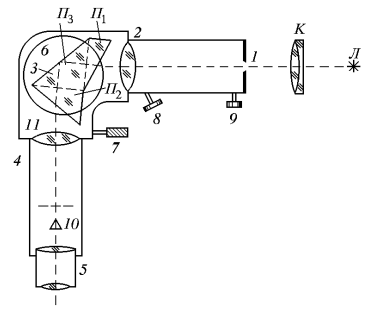
\includegraphics[width=0.6\textwidth]{img/scheme.png}
    \caption{Схема установки}
    \label{fig:scheme}
\end{figure}